% \preto\tabular{\setcounter{reqid}{0}}
\newcounter{reqid}
\newcounter{caseid}
\newcommand\req{%
  \stepcounter{reqid}%
  R-\padzeroes[3]{\decimal{reqid}}
}
\newcommand\reqcase{%
  \stepcounter{caseid}%
  C-\padzeroes[3]{\decimal{caseid}}
}
\newcolumntype{L}{>{\centering\arraybackslash}m{2.5cm}}

\chapter{An\'alisis de requisitos, dise\~no e implementaci\'on}\label{requisitos}

\section{Requisitos de información}
\subsection{Usuarios}
\begin{itemize}
  \item Nombre de usuario
  \item Contraseña
\end{itemize}
\subsection{Cartas}
\begin{itemize}
  \item Color
  \item Símbolo
\end{itemize}
\subsection{Partida}
\begin{itemize}
  \item Jugador del turno actual
  \item Cartas en la baraja
  \item Cartas en la pila de descartes
  \item Jugadores asociados
  \item Orientación de turnos
\end{itemize}
\subsection{Jugadores}
\begin{itemize}
  \item Cartas en mano
\end{itemize}


\section{Historias de usuario}
\subsection{Autenticación de usuario}

\subsubsection{Registro de usuario}

Como usuario sin autenticar, quiero poder registrarme en el sistema con un usuario y contraseña para poder acceder al juego. 

\subparagraph{Caso positivo} % (fold)

El usuario rellena un formulario en el que pone de nombre de usuario Pepito123 y contraseña MeGustanLosJabalies, tras hacer click en el botón de enviar, se mandarán los datos al servidor, que creará el usuario correspondiente e iniciará la sesión del usuario. 

\subsubsection{Inicio de sesión de usuario}

Como usuario sin autenticar, quiero poder usar mi usuario y contraseña para acceder a mi cuenta dentro de la aplicación y así acceder al juego. 

\subparagraph{Caso positivo}

El usuario sin autenticar, que se ha registrado anteriormente como Pepito123 y ha puesto de contraseña MeGustanLosJabalies, rellena un formulario en el que provee dichos datos, y tras darle al botón de enviar el sistema comprobará que la contraseña es la correcta para ese usuario y le dejará iniciar sesión. 

\subparagraph{Caso negativo 1}

Un usuario sin autenticar, que no se ha registrado anteriormente, provee en el formulario de inicio de sesión datos de usuario y contraseña que no existen en el sistema. El formulario se vuelve a mostrar, mostrando un mensaje de que los datos dados son incorrectos. 

\subparagraph{Caso negativo 2}

El usuario sin autenticar provee en el formulario un nombre correcto de usuario, pero pone una contraseña incorrecta. El formulario se vuelve a mostrar, con un mensaje mostrando que los datos introducidos son incorrectos. 

\subsection{Sala de espera}

\subsubsection{Crear una sala de espera }

Como usuario autenticado, quiero poder crear una sala de juego, para esperar a que otras personas entren antes de empezar el juego. 

\subparagraph{Caso positivo}

El usuario, tras autenticarse, hace click en un botón de “crear partida” y se le llevará directamente a una nueva sala de espera 

\subparagraph{Caso negativo }

El usuario, sin autenticar, hace click en un botón de “crear partida”, pero como no está autenticado, se le llevará a la página de autenticarse, indicando que debe iniciar sesión para crear la partida. 

\subsubsection{Unirse a una sala de espera }

Como usuario, quiero poder acceder a una sala de juego ya existente, para poder participar en el juego con los jugadores de dicha sala. 

\subparagraph{Caso positivo 1}

El usuario, tras autenticarse, hace click en un botón de “unirse a partida”, donde se le presentará un formulario donde podrá proveer el código de la partida, y una vez introduzca un código válido y le dé al botón de enviar, se le llevará a la sala de espera correspondiente 

\subparagraph{Caso positivo 2}

El usuario, tras autenticarse, usa un enlace que le ha dado el huésped de la partida que va a jugar, y al abrirlo se meterá automáticamente en la sala de espera 

\subparagraph{Caso negativo 1}

El usuario, sin autenticarse, hace click en un botón de “unirse a partida” y se le llevará a la página de autenticación, indicando que tiene que iniciar sesión. 

\subparagraph{Caso negativo 2}
El usuario, sin autenticarse, usa un enlace que le ha dado el huésped de la partida, y al abrirlo se le redirigirá a la página de autenticarse, indicando que tiene que iniciar sesión. 

\subparagraph{Caso negativo 3}
El usuario, tras autenticarse, pone en el formulario de unirse a una partida un código de una partida que no existe. Al darle click al botón de enviar, se le indicará que no existe esa partida y se le mostrará de nuevo el formulario. 

\subparagraph{Caso negativo 4}
El usuario, tras autenticarse, pone en el formulario de unirse a una partida un código de una partida que está en curso. Al darle click al botón de enviar, se le indicará que la partida está en curso y se le mostrará de nuevo el formulario. 

\subsubsection{Marcar estado de “listo” en sala de espera}

Como usuario, quiero poder marcar que estoy listo para empezar la partida, para así comunicar al huésped de la sala que puede comenzar la partida sin miedo a que yo me la pierda. 

\subparagraph{Caso positivo}

Un jugador no huésped le da a un botón de “Listo”, y para todos los demás jugadores y el huésped se les mostrará dicho estado. 

\subsubsection{Iniciar partida en sala de espera}

Como usuario y huésped en una sala de espera, quiero empezar la partida una vez haya observado que se han unido a la sala todas las personas que esperaba y que estén listas, para poder jugar con todas ellas. 

\subparagraph{Caso positivo}

El jugador huésped de una sala de espera, tras observar que todos los demás jugadores están listos para empezar la partida, hace click en un botón de Empezar Partida, y, tras ello, todos los jugadores serán redirigidos a la partida. 

\subsubsection{Configurar Reglas de la Casa}

Como usuario, al crear una sala de espera quiero poder escoger las reglas especiales a aplicar, para acomodar las preferencias mías y de mis compañeros al jugar. 

\subparagraph{Caso positivo}

El jugador huésped de una sala de espera hace click en la casilla de la regla de la intercepción para activarla durante la partida. 

Como jugador dentro de una partida, quiero poder especificar que digo “Uno” cuando me quedo con 1 carta en mano para poder cumplir con las normas del juego. 

\section{Matriz de trazabilidad de requisitos} % (fold)

\begin{longtable}{|L|L|L|L|L|}

\hline
ID de requisito & Descripción & ID de la prueba & Descripción de la prueba & Resultado esperado \\
\hline
\endhead

\hline
\endfoot


\req  &
  El usuario deberá poder registrarse e iniciar sesión en el sistema &
  \reqcase &
  El usuario sin autenticar ingresa datos correctos para iniciar sesión &
  El usuario inicia sesión correctamente \\
\cline{3-5}

 &
&
  \reqcase &
  El usuario sin autenticar ingresa datos incorrectos para iniciar sesión &
  El usuario no inicia sesión y se le muestra que no ha podido iniciar sesión \\
\cline{3-5}

&
  &
  \reqcase &
  El usuario sin autenticar ingresa datos correctos para registrarse &
  El usuario se registra en el sistema e inicia sesión, volviendo a la pantalla en la que estaba antes \\
\cline{3-5}

& &
  \reqcase &
  El usuario sin autenticar ingresa un nombre de usuario ya existente &
  El usuario no puede registrarse y se le informa que ese nombre de usuario ya existe                                                              \\
\hline


\req & El usuario podrá cerrar sesión en el sistema &
  \reqcase &
  El usuario autenticado hace click en un botón de cerrar sesión &
  El usuario cierra sesión correctamente \\
& &
  \reqcase &
  El usuario sin autenticar accede a la URL de cerrar sesión &
  No pasa nada \\
\hline


\req & El usuario podrá crear una sala de espera &
  \reqcase &
  El usuario autenticado hace click en crear sala &
  La sala se crea correctamente y el usuario se redirige a la nueva sala \\
\cline{3-5}

& &
  \reqcase &
  El usuario no autenticado hace click en crear sala &
  La sala no se crea y se redirige el usuario a la página de inicio de sesión, indicando que debe iniciar sesión \\
\hline

\req &
  El usuario podrá unirse a una sala de espera &
  \reqcase & El usuario autenticado escribe el código de sala y hace click en un botón de unirse                                                                               & El usuario se une a la sala correctamente y se redirige a la pantalla correspondiente                                                            \\
\cline{3-5}

 &
  &
  \reqcase &
  El usuario autenticado escribe el código de una sala que no existe y hace click en el botón de unirse &
  El usuario no se une a ninguna sala y se le muestra un error que le informa que la sala especificada no existe \\
\cline{3-5}

& &
  \reqcase &
  El usuario no autenticado escribe el código de una sala válida y hace click en el botón de unirse &
  El usuario se redirige a la pantalla de iniciar sesión, informándole que debe iniciar sesión \\
\hline


\req & El usuario dentro de una sala de espera podrá marcar que está listo para empezar &
  \reqcase &
  El usuario que no está listo dentro de una sala de espera hace click en un botón de “Listo” &
  El estado del usuario se actualiza a “listo” y se muestra a todos los usuarios en la sala \\
\cline{3-5}

&
  &
  \reqcase &
  El usuario que está listo dentro de una sala hace click en el botón de “Listo” &
  El estado del usuario se actualiza a “no listo” y se muestra a todos los usuarios en la sala \\
\hline

\req & El usuario anfitrión de una sala de espera podrá decidir comenzar el juego &
  \reqcase &
  El usuario anfitrión dentro de una sala de espera hace click en el botón de “Empezar partida”, estando los demás usuarios listos &
  El juego comienza con todos los usuarios siendo redirigidos como jugadores a la partida \\
\cline{3-5}

&
  &
  \reqcase &
  El usuario anfitrión dentro de una sala hace click en el botón de “Empezar partida”, pero un usuario no está listo &
  El juego no comienza, sino que se muestra un mensaje informando que todos los usuarios deben estar listos \\

\cline{3-5}
&
  &
  \reqcase &
  El usuario anfitrión dentro de una sala hace click en el botón de “Empezar partida”, pero no hay otros usuarios en la sala &
  El juego no comienza, sino que se muestra un mensaje informando que se necesitan más jugadores para iniciar el juego \\

\cline{3-5}
 &
  &
  \reqcase &
  El usuario no anfitrión dentro de una sala de espera intenta acceder a la URL de iniciar partida &
  El juego no comienza, sino que se muestra al usuario un error informándole de que no es el huésped de la sala \\
\hline

\req &
 El usuario podrá salir de una sala de espera, transfiriendo su rol de anfitrión a otro usuario si aplica &
\reqcase &
El usuario anfitrión dentro de una sala con otros usuarios hace click en el botón de “Salir” &
El usuario se elimina de la sala y el rol de anfitrión se transfiere a cualquier otro usuario de la sala \\

\cline{3-5}
&
  &
  \reqcase &
  El usuario no anfitrión dentro de una sala de espera hace click en el botón de “Salir” &
  El usuario se elimina de la sala \\
\hline

\req & Al salir el último usuario de una sala de espera, esta se borrará &
  \reqcase &
  El único usuario dentro de una sala de espera hace click en el botón de “Salir” &
  La sala se borra \\
\hline

\req & El usuario anfitrión de una sala de espera podrá escoger las reglas de la casa con las que jugar &
  \reqcase &
  El usuario anfitrión dentro de una sala de espera hace click en una checkbox correspondiente a la regla de intercepción &
  Se configura la partida a crear para tener habilitada la regla de intercepción \\
\cline{3-5}

&
  &
  \reqcase &
  El usuario anfitrión de una sala de espera no habilita ninguna regla &
  La partida se iniciará sin ninguna regla especial habilitada \\
\hline

\req & Las reglas del juego deberán cumplirse dentro de una partida &
  \reqcase &
  Se comienza una partida con varios jugadores &
  Se entregarán 7 cartas a la mano de cada jugador. Se pone una carta en la pila de descartes. \\
\cline{3-5}

&
  &
  \reqcase &
  En una partida, comienza el turno de un jugador &
  Se le entrega una carta de la baraja \\
\cline{3-5}

&
  &
  \reqcase &
  En una partida, todos los jugadores se quedan sin cartas excepto 1 de ellos &
  Se termina la partida \\
\hline

\req & El usuario dentro de una partida deberá poder jugar cartas &
  \reqcase &
  En una partida, en el turno de un jugador, este escoge una carta con el mismo color o símbolo que la de la pila de descarte &
  La carta se mueve de la mano del jugador a la pila de descartes \\
\cline{3-5}

&
  &
  \reqcase &
  En una partida, en el turno de un jugador, este escoge jugar una carta de distinto número y símbolo que la de la pila de descarte, haciendo click en ella &
  La carta no se juega \\
\cline{3-5}

&
  &
  \reqcase &
  En una partida, un jugador intenta jugar una carta haciendo click en ella fuera de su turno &
  La carta no se juega \\
\cline{3-5}

&
  &
  \reqcase &
  En una partida, un jugador juega un comodín durante su turno &
  La carta se mueve correctamente y se le pide al jugador escoger un color                                                                         \\
\cline{3-5}

&
  &
  \reqcase &
  En una partida, un jugador juega una carta de robar cartas &
  El siguiente jugador en el orden de turnos recibirá el número indicado de cartas del mazo según la carta jugada indique y su turno será omitido  \\
\cline{3-5}

&
  &
  \reqcase &
  En una partida, un jugador juega una carta de omitir turno &
  El turno del siguiente jugador será omitido \\
\cline{3-5}

&
  &
  \reqcase &
  En una partida, un jugador juega una carta de invertir orden de turnos &
  El orden de turnos se invertirá de horario a antihorario o viceversa \\
\hline

\req & El usuario dentro de una partida podrá robar cartas cuando sea necesario &
  \reqcase &
  En una partida, en el turno de un jugador, este decide robar una carta &
  El jugador recibirá una carta del mazo \\
\cline{3-5}

&
  &
  \reqcase &
  En una partida, en el turno de un jugador, este ha robado una carta carta jugable y decide jugarla &
  El jugador jugará esa carta de su mano y se pondrá en la pila de descartes \\
\cline{3-5}

&
  &
  \reqcase &
  En una partida, en el turno de un jugador, este ha robado una carta jugable de la baraja y decide no jugarla &
  El jugador deberá robar una carta más de la baraja y pasar su turno al siguiente jugador \\
\cline{3-5}

&
  &
  \reqcase &
  En una partida, en el turno de un jugador, este ha robado una carta no jugable &
  El jugador no podrá jugar la carta, por lo que tendrá que robar una carta más y pasar su turno \\
\cline{3-5}

&
  &
  \reqcase &
  En una partida, en el turno de un jugador, este ha robado una carta e intenta jugar otra carta desde su mano &
  La carta no se juega. \\
\hline

\req & El usuario dentro de una partida deberá poder anunciar que le queda una única carta &
  \reqcase &
  En una partida, en el turno de un jugador con 2 cartas, con al menos una de ellas jugable, decide anunciar que le queda una carta &
  Se marca que el jugador ha anunciado correctamente \\
\cline{3-5}

&
  &
  \reqcase &
  En una partida, en el turno de un jugador con 2 cartas no jugables, decide anunciar que le queda una carta &
  El anuncio no se realiza. \\
\cline{3-5}

&
  &
  \reqcase &
  En una partida, en el turno de un jugador con 2 cartas, al menos una de ellas jugable, anuncia que le queda una carta y decide robar una carta &
  La carta no se roba. \\
\hline

\req & El usuario dentro de una partida podrá acusar a otros jugadores para cumplir ciertas normas &
  \reqcase &
  En una partida, un jugador, tras jugar una carta se queda con una única carta en su mano, no lo anuncia y otro jugador lo acusa &
  El jugador acusado debe robar 2 cartas \\
\cline{3-5}

&
  &
  \reqcase &
  En una partida, un jugador con 2 cartas juega una de ellas, no lo anuncia, el turno del siguiente jugador termina y otro jugador acusa al primero de no decir uno &
  No ocurre nada \\
\cline{3-5}

&
  &
  \reqcase &
  En una partida, un jugador juega un comodín de robar 4 cartas teniendo otras cartas jugables de otro tipo y otro jugador lo acusa de ello &
  El acusado roba 4 cartas, y el siguiente jugador en el orden de turnos no tiene que saltarse su turno ni robar las cartas especificadas \\
\cline{3-5}

&
  &
  \reqcase &
  En una partida, un jugador juega un comodín de robar 4 cartas sin tener otras cartas jugables de otro tipo y otro jugador lo acusa de ello &
  El jugador acusador roba 6 cartas, y el siguiente jugador en el orden de turnos no tiene que saltarse su turno ni robar las cartas especificadas \\
\hline

\req &
  El usuario dentro de una partida deberá poder escoger el color a aplicar al jugar un comodín &
  \reqcase &
  A &
  A \\
\hline

\req &
  El usuario deberá poder anunciar que le queda una sola carta en mano &
  \reqcase &
  A &
  A \\
\hline


\req &
Las reglas de la casa deberán tener efecto si están activadas para la partida &
\reqcase &
 & 

\end{longtable}

% section  (end)

\section{Dise\~no e implementaci\'on}

\subsection{Arquitectura del sistema}

Se realizará una arquitectura por capas compuesta por:

\begin{itemize}
  \item Capa de presentación
  \item Capa de servidor
  \item Capa de datos
\end{itemize}

\subsubsection{Capa de datos}
Se realizará usando MongoDB para una base de datos NoSQL,
debido a que puede acomodar más fácilmente la estructura del juego,
comparado con una base de datos relacional.

Esto también resulta en mayor rendimiento, ya que se evitan operaciones de unión de tablas.

\paragraph{Esquema de la base de datos}

\begin{center}
  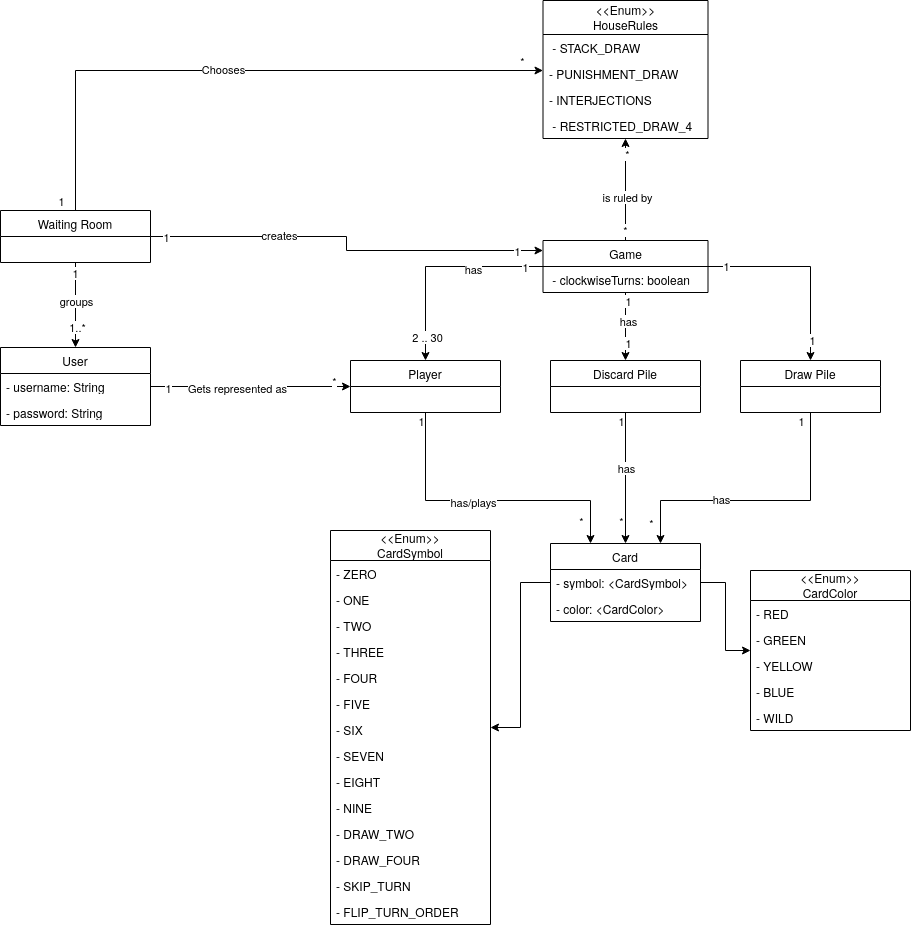
\includegraphics[width=1\textwidth]{img/BD_drawio.png}
  \captionof{figure}{Representación UML de la base de datos} \label{fig:dbschema}
\end{center}

\subsubsection{Capa de servidor}
Se creará en lenguaje JavaScript debido a la familiaridad con el mismo, aunque se añadirá al mismo tiempo TypeScript. 

Al mismo tiempo, se incorporará Bun,
ya que provee mayor rendimiento y soporte nativo para TypeScript,
así como otras funcionalidades como la ejecución de tests. 

Como framework, se hará uso de Elysia como framework de Backend, ya que está intencionado para su uso con Bun. 

\paragraph{Documentación de la API:}

La API del servidor se documentará con las especificaciones de OpenAPI para las rutas normales y AsyncAPI para las rutas con WebSockets.
La estructura consistirá de las siguintes rutas:

\subparagraph{Rutas de la API REST:}

\begin{itemize}
  \item /user
    \begin{description}
      \item[POST:] Registra un nuevo usuario
        \begin{description}
          \item[username:] Nombre de usuario
          \item[password:] Contraseña
        \end{description}
    \end{description}
    \begin{itemize}
      \item /login
        \begin{description}
          \item[POST:] Inicia sesión del usuario
            \begin{description}
              \item[username:] Nombre de usuario
              \item[password:] Contraseña
            \end{description}
        \end{description}
    \end{itemize}
  \item /room
      \begin{description}
      \item[POST:] Crea una sala de espera nueva asociada al usuario actual
      \end{description}
\end{itemize}
\subparagraph{Rutas de la API WebSockets:}
% TODO: Add Websocket API routes
\begin{itemize}
  \item Test
\end{itemize}

\subsubsection{Capa de presentación}

Se realizará también con JavaScript y Bun, por razones similares a las de la capa de servidor. 

Se usará el framework de React debido a su gran cantidad de documentación y popularidad, así como por la experiencia previa que se ha tenido con dicho framework. 

Adicionalmente, otras tecnologías que se usarán en este apartado son Vite para utilidades de desarrollo, y Tailwind y la librería de primitivos de Radix. 

Tailwind se ha escogido debido a que simplifica el proceso de diseño de estilos, y gracias a los componentes de React se pueden abstraer y reutilizar fácilmente a través de toda la aplicación. 

La librería de primitivos de Radix, considerada una librería de componentes “headless”, se ha escogido debido a que provee componentes funcionales sin estilo, con un enfoque en la customización. 

\paragraph{Mockups}

\begin{center}
  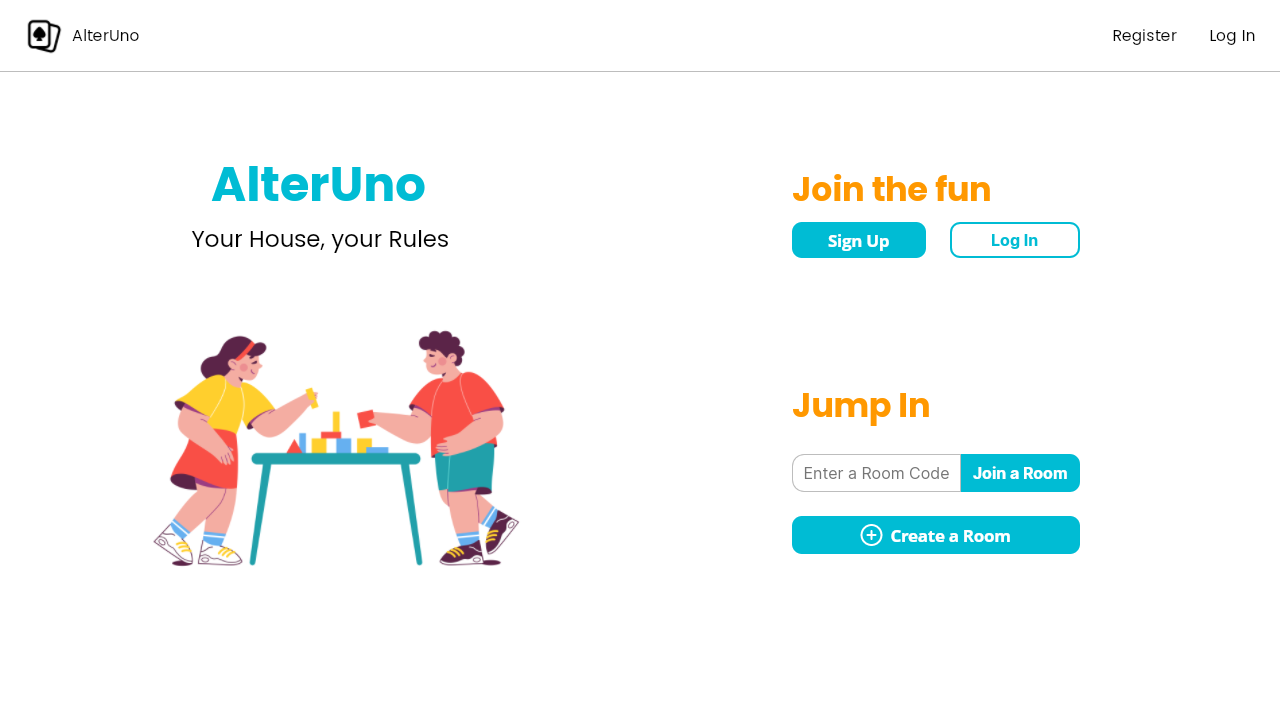
\includegraphics[width=1\textwidth]{img/Mockup Main Page}
  \captionof{figure}{Mockup de la pantalla de inicio} \label{fig:mainmockup}
\end{center}

\begin{center}
  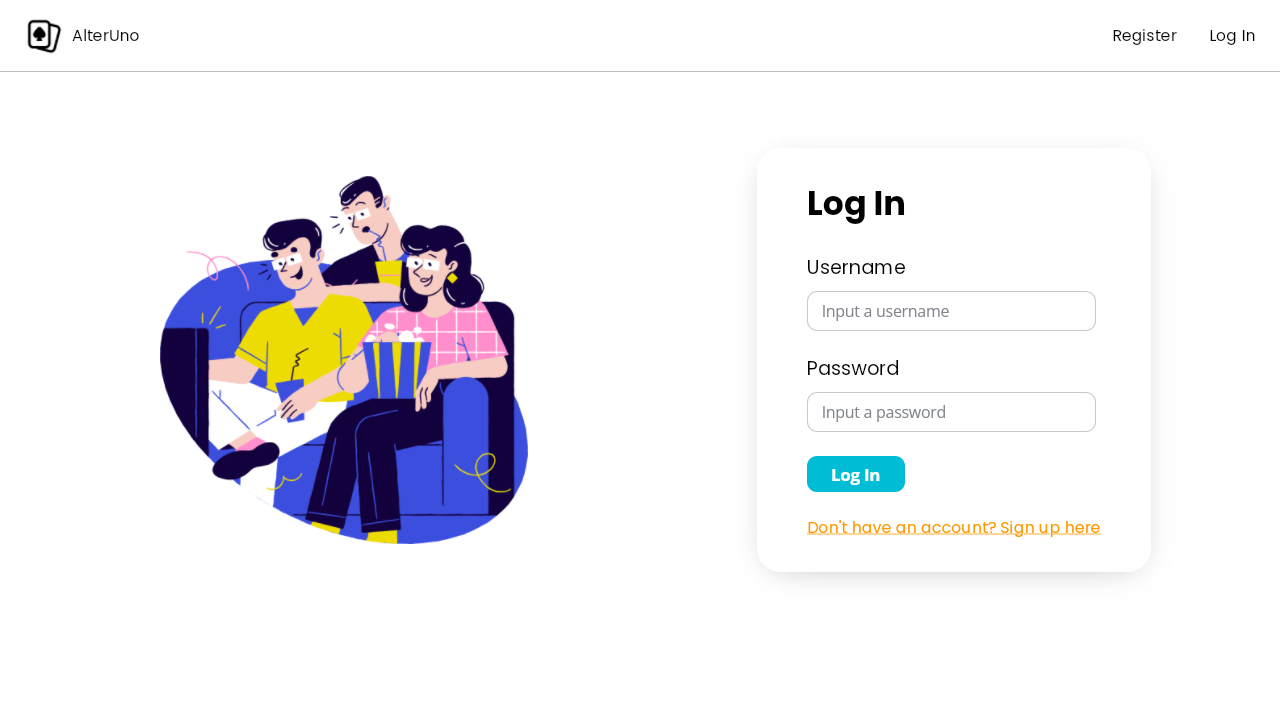
\includegraphics[width=1\textwidth]{img/Mockup Log In}
  \captionof{figure}{Mockup de la pantalla de inicio de sesión} \label{fig:loginmockup}
\end{center}

\begin{center}
  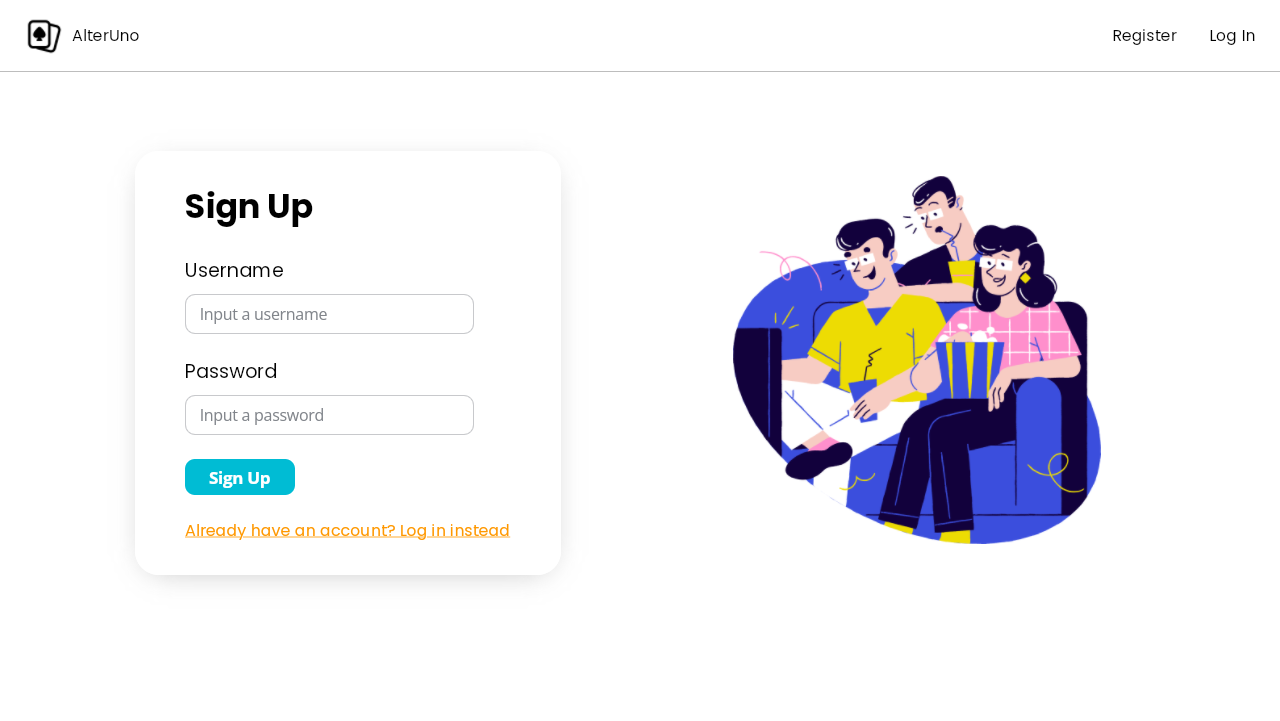
\includegraphics[width=1\textwidth]{img/Mockup Sign Up}
  \captionof{figure}{Mockup de la pantalla de registro} \label{fig:signupmockup}
\end{center}

\begin{center}
  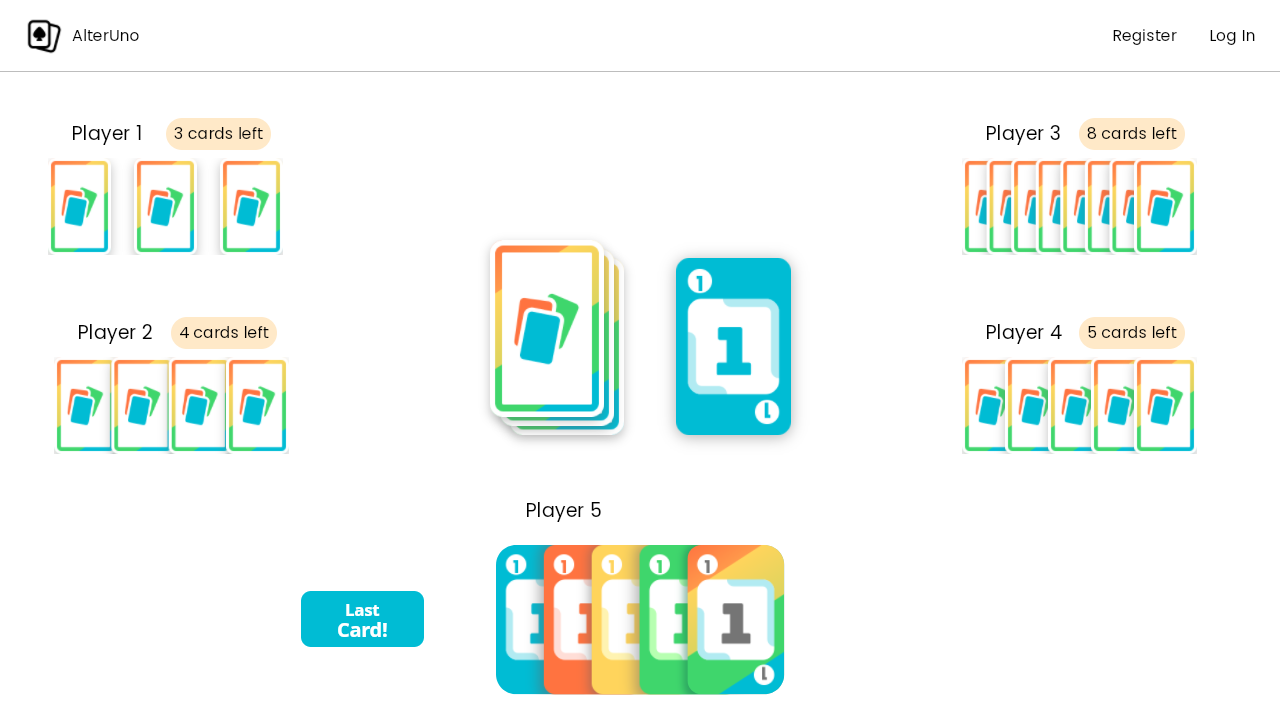
\includegraphics[width=1\textwidth]{img/Mockup Game}
  \captionof{figure}{Mockup de la pantalla del juego} \label{fig:gamemockup}
\end{center}


